\documentclass[10pt,journal,draftcls,onecolumn]{IEEEtran}
\usepackage{CJKutf8}
\usepackage{graphicx}
\usepackage{subfigure}
\usepackage{amsmath}

\usepackage{graphicx}

\usepackage{listings}
%\makeatletter
%\let\@square\relax
%\makeatother
%\usepackage{SIunits}            % typset units correctly
\usepackage{courier}            % standard fixed width font
\usepackage[scaled]{helvet} % see www.ctan.org/get/macros/latex/required/psnfss/psnfss2e.pdf
\usepackage{url}                  % format URLs
\usepackage{listings}          % format code
\usepackage{enumitem}      % adjust spacing in enums
\usepackage{color}
\usepackage{xcolor}
\usepackage{caption}
%\usepackage{hyperref}
\usepackage{multirow}

\begin{document}

\begin{CJK*}{UTF8}{gbsn}
\title{代码片段分析与标签预测}

\author{
\alignauthor 2120151009 廖心怡\\
\affaddr{嵌入式高性能计算实验室, 北京理工大学}\\
\email{suiyi528@163.com}\\
\and
\alignauthor 2120150983 扶聪\\
\affaddr{计算机学院, 北京理工大学}\\
\email{416310463@qq.com}
}
\date{July 2016}

\maketitle

\section{简介}
代码片段是指在源文件中无论何时何地我们需要就可以被重用的一段源代码。代码片段可以非常短,比如一行源代码,或者非常复杂,比如一整个类和方法。虽然在代码片段的变量名可以在不同环境下的变化,但其轮廓通常是保持不变的。代码片段可能是源代码模板,直接重用以减少需要键入的文字,可能是如何使用API或数据结构,也有可能仅仅是实现特定的功能块一个简单的例子。

在本文中,我们代码片段进行分析与标签预测。我们在现实世界的代码里有一个彻底的调查并且使用标签来标记代码片段。我们展示如何使用一个训练片段分类模型来标记代码片段,然后对代码片段进行标签预测。

\section{问题陈述}
一个有经验的程序员可能会在他/她的编程生涯中做过许多的项目,并且总是在不同的项目场景中实现相同的功能。以文件打开操作为例,这个功能非常必要并且几乎出现在每个真实应用中。程序员每次遇到这种情况时需要把这些代码记在脑中并且用自己的代码风格将这段代码码出来。一个程序员可能在不同的项目中一遍又一遍地实现相同的功能,但是由于程序语言本身并不提供一个机制来保存一个程序员自己格式化后的代码片段,并且从以前的项目中复制过来并不高效,因为需要花更多的时间来进行查找以及来对代码的语法进行校正,对代码中的一小段在不同时间不同地点的功能验证。

在一般情况下,代码片段被程序员提交到他们的网页博客上,保存在文本文件中或者存储在系统中,并且预计它们在一段时间后会被重用。由于熟练地管理和片段的重复使用可显著提高实践中的编程效率,有经验的程序员通常有自己的代码片段存储库并且他们每个人都有不同的方法来管理代码片段。代码片段管理也是一些文本编辑器、程序的源代码编辑器和集成开发环境的某个功能。不幸的是,根据以往的经验和我们的调查结果表明,片段重用和共享并不像预期的那样有效,这一事实违背片段重用的主要目标。

这尴尬的情况是由许多原因造成的,但我们认为,其中一个主要原因是片段并没有很好的标记方法。以gist为例,每天大约有3000个片段公布在gist上,但是只有平均35$\%$的片段代码存在文本描述。此外,大多数的描述是不超过十个字的。这部分是由于程序员匆忙地将片段提交给管理系统,但主要是因为目前的管理系统不提供一个有效的标签框架。一些片断管理系统鼓励程序员使用用户定义的标签标注自己的片段。在一定程度上,一个片段也可以自动地通过基于一个大的库统计分析的管理系统进行标记。关键词标签在片段索引和检索中是有用的,但它不是一个可以用来在程序员之间共享代码片段的常见和公共的标准,更不用说不同的管理系统中了。

片段管理现阶段并不像预期的那样有效,原因包括以下几点:
\begin{itemize}
    \item 离线个人片段收集及管理是十分麻烦的,因为片段以各种形式保存在不同的位置中。程序员都是怕麻烦的,他们并不不喜欢陷入琐事中,如合并、版本管理、转移和索引。
    \item 出现在用户的博客中的代码片段都是有着丰富的文本描述的,但是他们只能在其所在博客被搜索引擎搜索到并且排位比较靠前的时候才能被其他人发现和重用。此外,程序员为他们的问题寻找合适的关键字需要花费一些时间,从搜索引擎返回的列表中找到合适的结果也会耗费一些时间。
    \item 片段关键字标记搜索和检索中,某种程度上是有用的,但这并不是一个正式的明确描述的概念域。程序员与程序员之间、程序员和系统之间共享或者共同理解片段依旧是个问题。
\end{itemize}
\section{技术方案}
\subsection{代码片段的爬取}
我们使用网络爬虫技术将gist@GitHub和code@CSDN中的代码爬取出来。首先我们找到相应的URL,由于每一个代码片段的页面布局是一致的,而它们在网站中有一个自己的唯一的id。我们编写了一个爬虫程序,每次运行时设定一个id的初始值,然后对于每一个id对应的网页,程序首先将网页保存到本地,然后自动获得代码片段的名称、源代码片段、标签、描述、上传时间等等数据并存入数据库。然后我们就能对这些代码片段进行分析了。

\subsection{代码片段标注与预测}
\subsubsection{特征提取}
首先,将描述划分成单个的字或者词。然后,描述中的每一个词都当做代码片段中的一个特征,所有的词形成一个特征集Fd。接下来,将源代码中的每一个词都都当做代码片段的一个特征,然后从源代码中提取的所有特征值形成的特征集为Fc。虽然代码片段中的词数通常都小于文本文档,但是潜在的特征值数量往往会超过训练集代码片段的数量。特征提取是整个过程的第一步,用来将代码片段表示成清晰的文字格式。代码片段是由大量的单字表示,大部分的代码片段都是繁杂的。描述中的标点符号,分隔符,运算符,常量和标识符都会在预处理中被移出。源代码中的英文单词和Java的包名和类名都会成为特征向量空间的一部分。代码片段的特征集F的定义为:

\begin{equation}\label{equation_element}
F=F_d\cup F_c
\end{equation}

\subsubsection{特征选择}
在文本分类中最重要的困难时特征空间具有高维度,因为文档中可能包含成百上千个不同词汇。一些学习算法可以处理这么大的输入特征,但是这些算法清冽的系统能够在不牺牲分类精确度的情况下能够减少本地空间[14]。在代码片段进行预处理之后,特征选择是指通过单词的重要性选出得分最高的单词作为特征的子集。近年来已经有许多特征选择技术被提出并且自动选择的目标已经被实现。每一种文本分类技术都有它的优缺点,为了找到哪一种特征选择方法可以在代码片段分类中具有高的准确率,6种常用的特征选择方法将用来进行对比。下面将对每一种方法来进行说明: 
\begin{itemize}
    \item 互信息(MI):互信息衡量某个词与类别之间的独立关系。它测量一个信息的存在/不存在对做出正确的分类决定有多少贡献。
    \item 信息增益(IG):信息增益是通过查看一个信息出现时和没有出现时的熵的变化,来判断一个特性是否重要。也就是说,它的衡量标准在于看特征能够为该分类系统带来多少信息,特征的重要程度与带来的信息量息息相关。
    \item 卡方检验(CHI-square):卡方检验[14]是用于统计数据中,测试两个事件的独立性。具体而言,放在特征选择这一块,它测试一个特性术语的出现与一个特定类的出现是否是独立的。
    \item 加权频率和概率(WFO):加权频率和概率[15]是一个特征选择方法,它可以适当的调整两个测量值的倾向。在WFO中,好特征的定义是指在文档中出现频率高且类别比率高的特征。WFO的公式中具有一个参数,通过调整这个参数的值,我们可以调整每一个测量值的偏好来得到好的特征值,当这个参数的值为0.5时,这个算法就是WLLR算法。
    \item 加权日志可能性定量(WLLR):WLLR偏向于高类别比率和高文档频率的术语,在WLLR中,频率测量似乎要比比率测量具有更重要的地位。
    \item 术语频率-逆文档频率(TF-IDF): TF-IDF是经典的信息检索词权重模型。它通过使文档中术语的原始术语频率和和文档中术语的逆文档频率相乘来估计给定文档中的术语的重要性。
\end{itemize}



\subsubsection{特征屏蔽}
由于我们使用了描述和源代码进行了文本分类,从之前的表3-1我们可以知道,特征提取出的向量中一定会出现一些与分类无关的词汇(如leetcode)。由于这些词汇本身出现与该代码片段注释毫无关联。如果不屏蔽掉这些词汇的话,可能会出现下面的情况:一个代码片段分类到A,其中出现了较多无关词汇,此时另一个代码片段本应分类到B,但是由于同样出现了与第一个代码片段相同的无关词汇,结果被模型分类到了A。这种情况的后果就是大大降低了我们模型分类的准确率,与我们本课题的目的相左。

另一种词汇就是几乎在每段代码片段或者描述中都出现的词汇,这些词汇本身是与分类相关的,但是由于几乎在每个代码片段中出现,对分类来说这类词汇的存在的影响挺大,可能一不小心就会使片段代码分错类。

我们需要将上述两类的词汇屏蔽掉,由于这些词语数量级并不是特别大,我们采用手动添加屏蔽词汇的方法,我们一共屏蔽了约200个无关词汇。

\subsubsection{特征训练}
和文本分类相似,每一个代码片段都可以用一个向量$\vec{s}$来表示,它的第k个元素的频是:
\begin{equation}\label{equation_element1}
f(x_k^s)=\begin{cases}
    0 \quad \quad \quad  x_k^s\not\in F \\
    1 \quad \quad \quad  x_k^s\in F \\
  \end{cases}
\end{equation} 

每一个类都是由一个向量$\vec{c}$表示,它的第k个元素表示为:
 \begin{equation}\label{equation_element2}
u_k^c=\frac{n_k^c}{n_k}\times \alpha^{w_k^c}\times W(c,k)
\end{equation}
其中,$n_k^c$是指训练集中属于c类的第k个元素的数目,$n_k$是指所有类中第k个元素的总数目,$w_k^c$是指在类c中第k个值的权重,参数$\alpha$是使用手动调整或者使用交叉验证的。而W(c,k)的定义为:
\begin{equation}\label{equation_w}
W(c,k)=\begin{cases}
    N_d^c/N^c*\beta_d \quad \quad \quad  x\in F_d  \\
    N_p^c/N^c*\beta_c \quad \quad \quad  x\in F_c  \\
  \end{cases}
\end{equation}
其中, $N_d^c$是指从训练集的Fd中选出的特征属于类c的数量, 是指训练集中源代码里选出的特征属于类c的数量, $N^c$ 是$N_d^c$与$N_c^c$ 之和。 $\alpha_m$和$\alpha_s$都是可以手动调整的参数。


\section{实验与实现结果}
\subsection{代码片段的统计与分析}
从gist@GitHub上爬取得数据和从code@CSDN上爬取得数据在很多地方上是不同的。首先,用户上传到gist@GitHub上的大多数代码片段有很少或者根本没有描述,提供的分类信息也是少的可怜。相比之下,大多从code@CSDN上获得的代码片段都是从有深厚开发经验的用户博客中获取的,博客提供一个平台让他们用丰富的语言来描述他们的源代码。表~\ref{table_snippets}是我们对两个网站获取的代码片段进行的对比。我们对gist@Github的中数据进行了7周的爬取工作,每天爬取两到三次数据,大概爬取到1300个代码片段,最后得到了git@GitHub数据集。code@CSDN由于刚刚经历过网站的列表整合,所以在15天内我们访问了超过10,000条的数据。但是由于code@CSDN上的数据的创建日期都不会显示在原网站上,所以我们无法知道这些片段是什么时候创建的。

\begin{table}
  \centering
  \caption{代码片段属性}
  \begin{tabular}{ccccc}
    \hline
    % aftBackus:60er \\: \hline or \cline{col1-col2} \cline{col3-col4} ...
    特征                & gist@GitHub       & code@CSDN  &  & \\
    \hline
    标题                   & 很少               & 没有        &  &  \\
    描述             & 很少               & 很多      &  &  \\
    标签                     & No                & 很多      &  &  \\
    描述语言       & 英语和其他语言  & 中文   &  &  \\
    来源                 & 用户提交的            & 网站整合的 &  &  \\
    代码数量            & 65k              & 145k       &  &  \\
    用户数量               & 35k              & 36k        &  &  \\
    \hline
  \end{tabular}
  \label{table_snippets}
\end{table}
图~\ref{gist_size}显示了从gist@GitHub和code@CSDN中的代码片段大小分布。不出所料的,代码片段总体来说都是小型的并且含有100行源代码,大多数的代码片段有少于200行的源代码,而且这个数字还包括空行和说明。从我们得到的数据集来看,code@CSDN中大约有72.6$\%$的代码片段是少于100行源代码的,这一比率在gist@GitHub还要更高一点。
\begin{figure}
\centering
  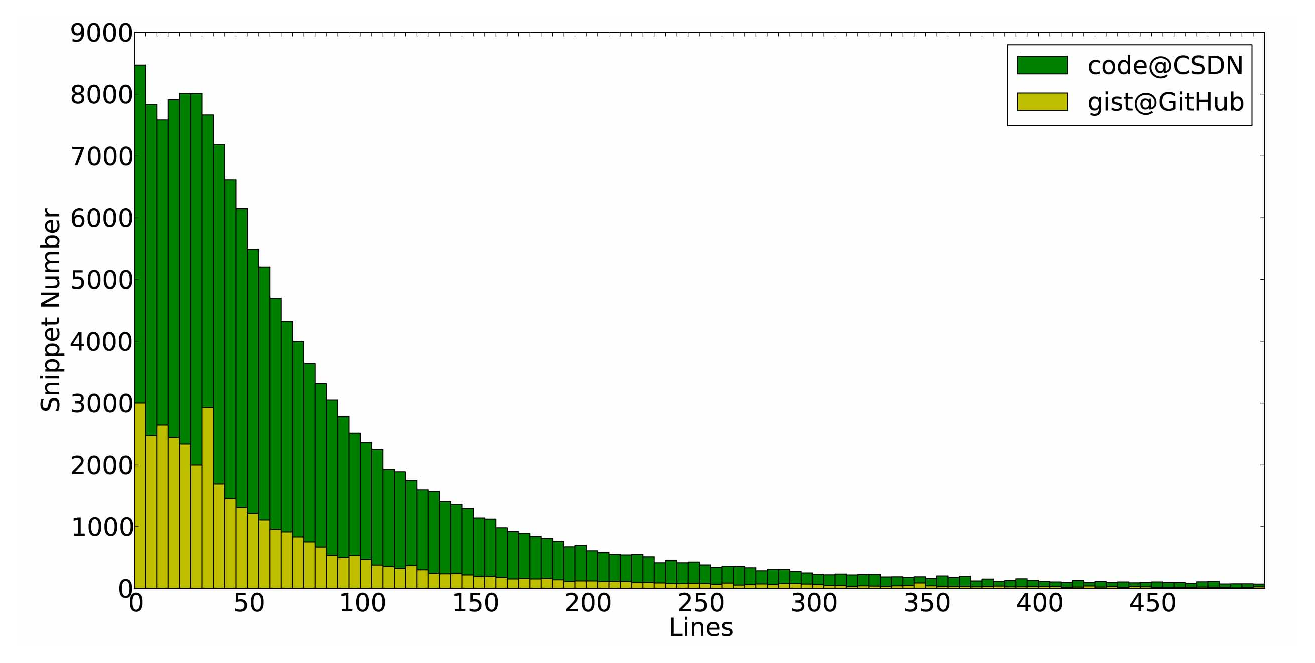
\includegraphics[height=1.5in, width=3in]{lines.eps}
  \caption{从gist@GitHub和code@CSDN上爬取的代码大小的分布}\label{gist_size}
\end{figure}

图~\ref{gist_programmer}显示了在我们的数据集中同一个程序员上传到gist@GitHub和code@CSDN的代码片段数量。由于code@CSDN中获取的代码片段的时间跨度更大,所以平均每个用户贡献了更多的代码片段。但是在我们的数据集中有一个不可否认的事实是大量的用户只提交了几个代码片段。这意味着虽然代码管理的需求是强烈的,但是这两个系统中的大多数用户在使用系统中表现的并不活跃。
\begin{figure}
\centering
  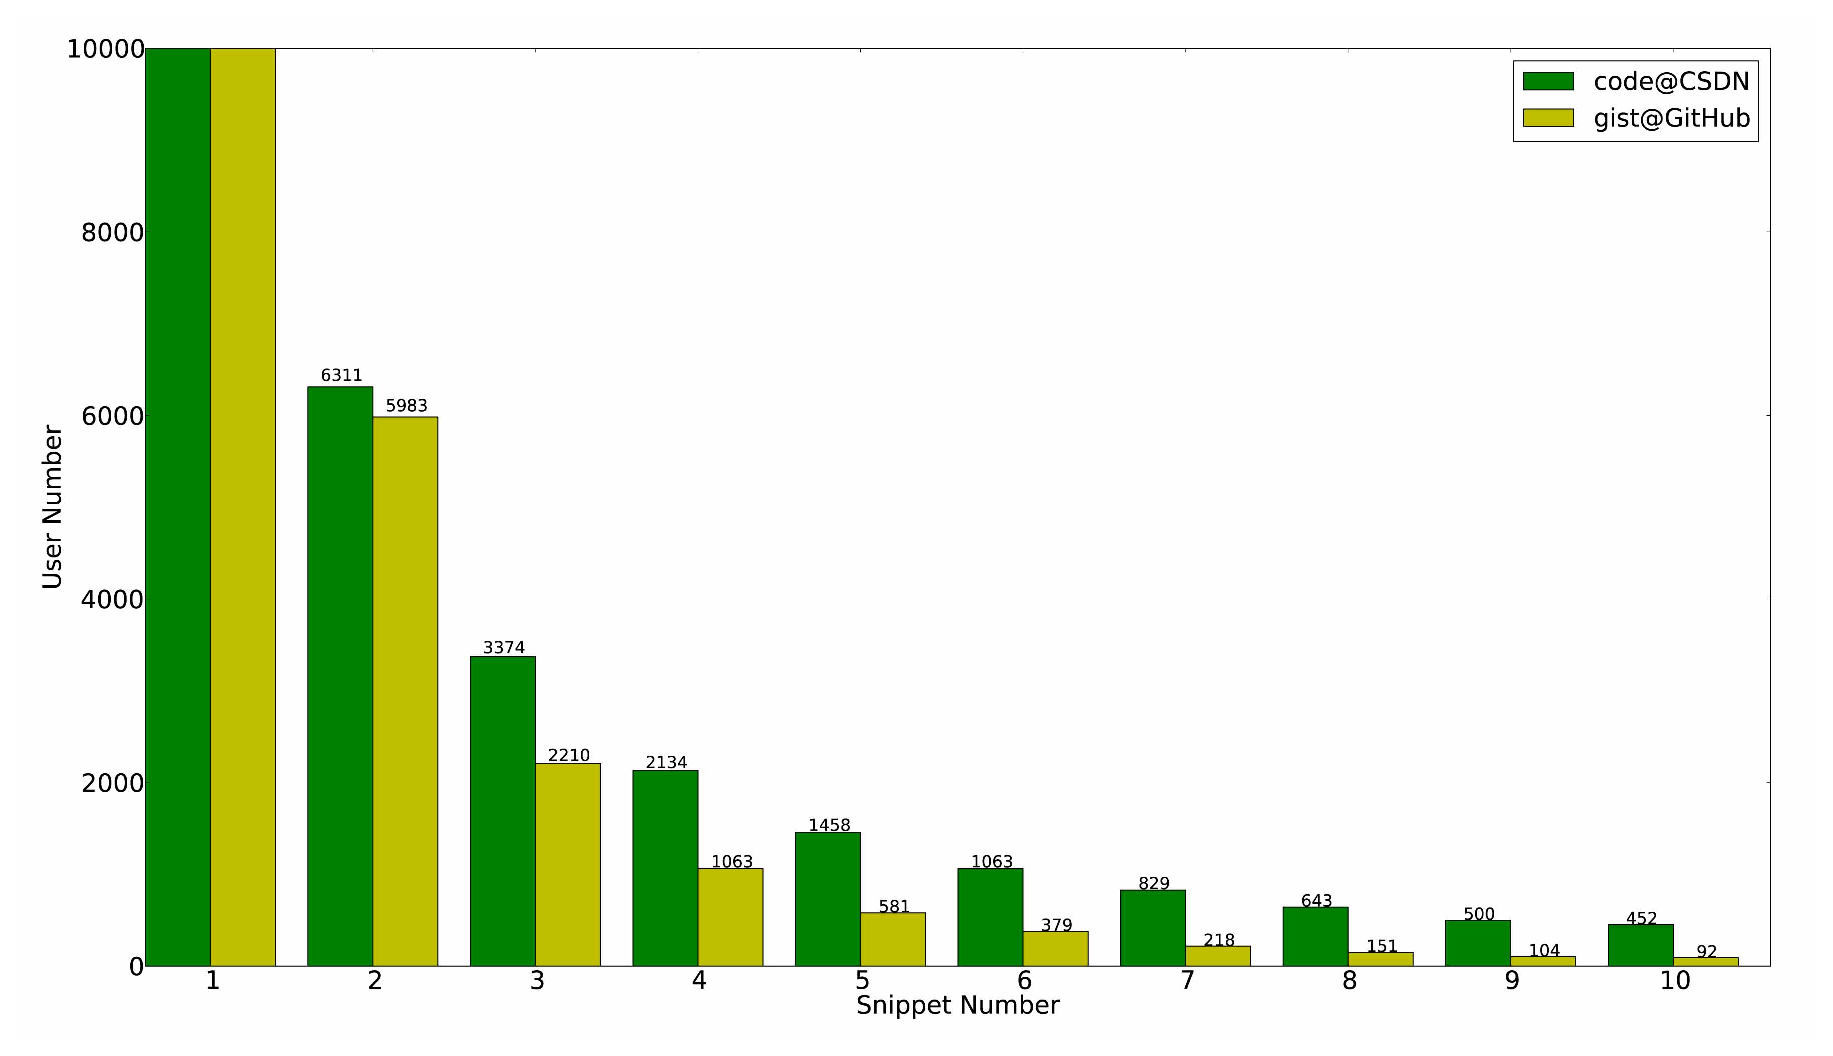
\includegraphics[height=1.5in,width=3.4in]{user.eps}
  \caption{程序员提交的代码片段数量}\label{gist_programmer}
\end{figure}

图~\ref{snippet_language}是代码片段的语言分布图。它表明了语言的片段是否受欢迎是随地区而定的。例如,C++,Java,SQL
和C$\#$在ode@CSDN更受欢迎然而JavaScript(图中的JS)、Python、C、PHP、CSS、Ruby在Gist@GitHub上更受欢迎。脚本语言,比如JavaScript、Python和PHP,显然是gist@GitHub用户最为喜欢的语言。

\begin{figure}
\centering
  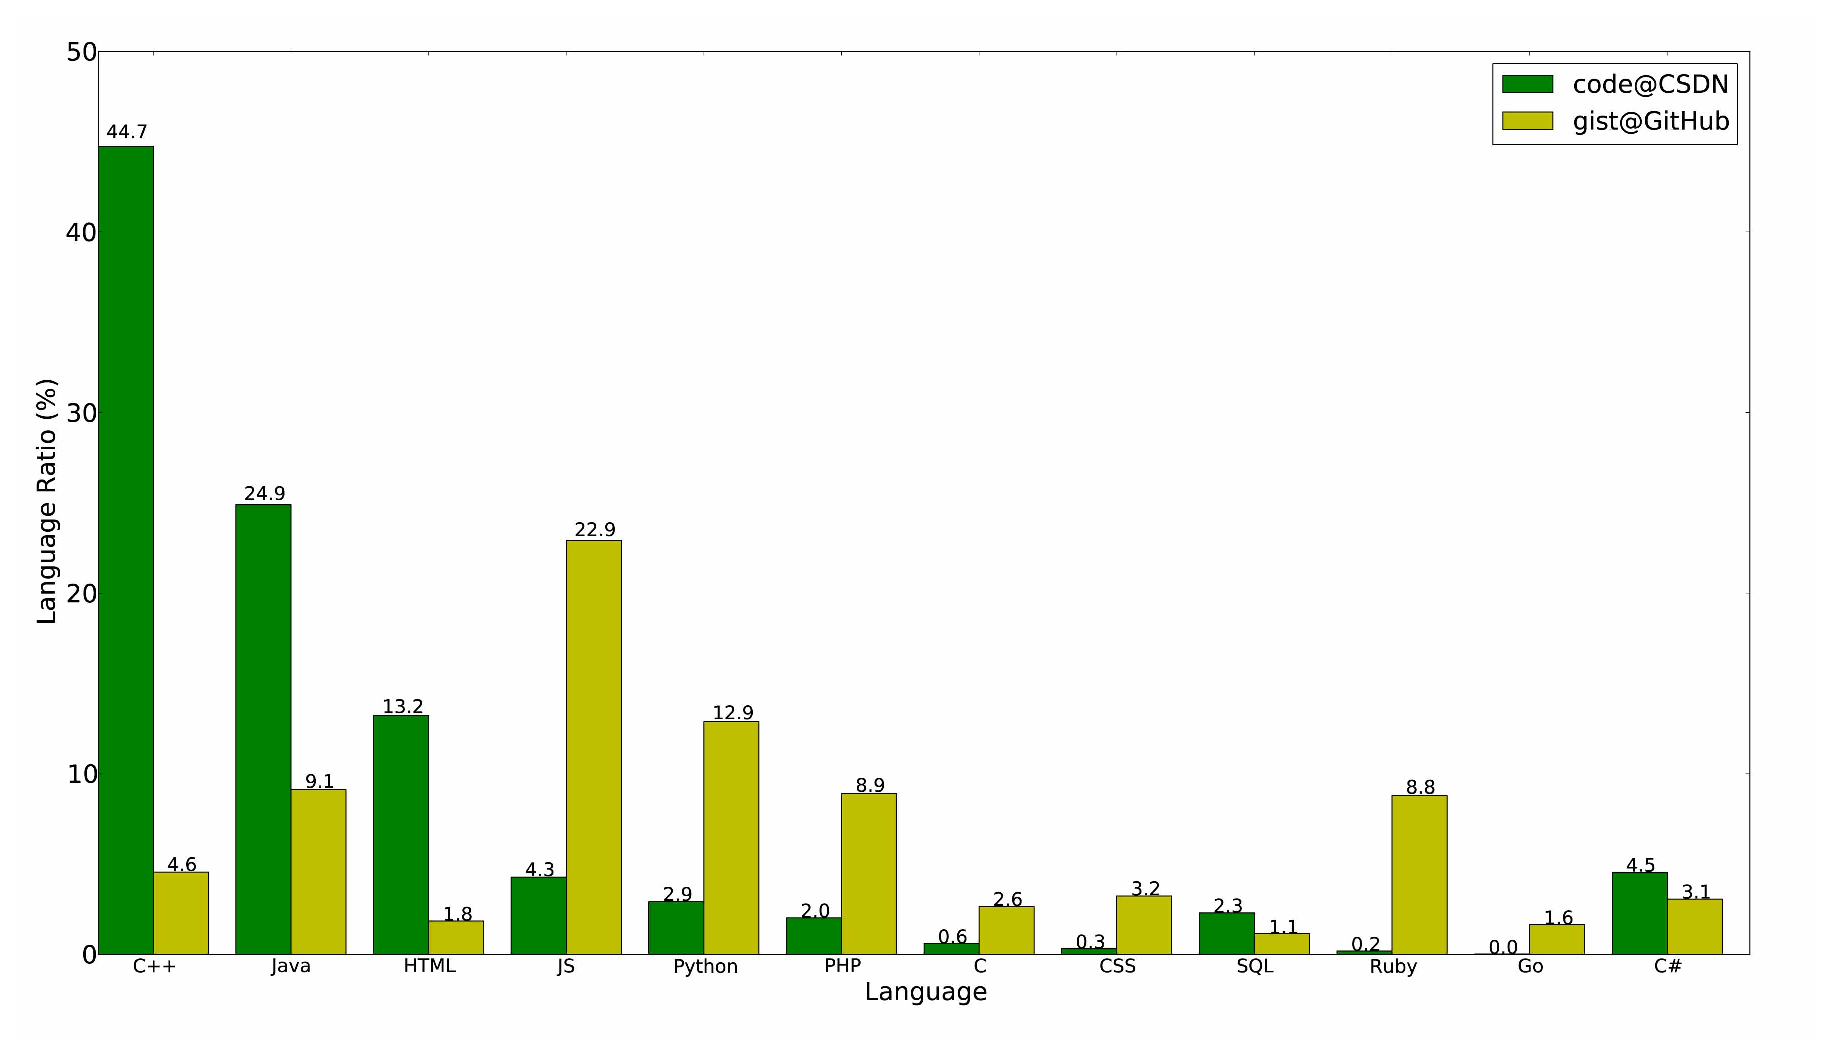
\includegraphics[height=2in,width=3.4in]{languages.eps}
  \caption{不同语言的代码片段分布情况}\label{snippet_language}
\end{figure}

最后一幅图也就是图~\ref{snippet_description}展示了代码片断的描述字数长度。由于gist@GitHub是一个国际性的平台。来自许多国家的人在提交他们的片段是会采用多种语言来描述。大部分的片段都是没有描述的,97$\%$的片段的描述少于10个字。根据我们的经验和一些小调查,这种情况发生的原因在于很多时候程序员都是匆匆忙忙地将代码片段上传到在线系统中。这意味着一个高效的标签框架对于代码片段的提交和重用是十分有必要的。一个自动注释的机制将会在这个过程中非常有用,因为它大大减少了注释的时间。
\begin{figure}
\centering
  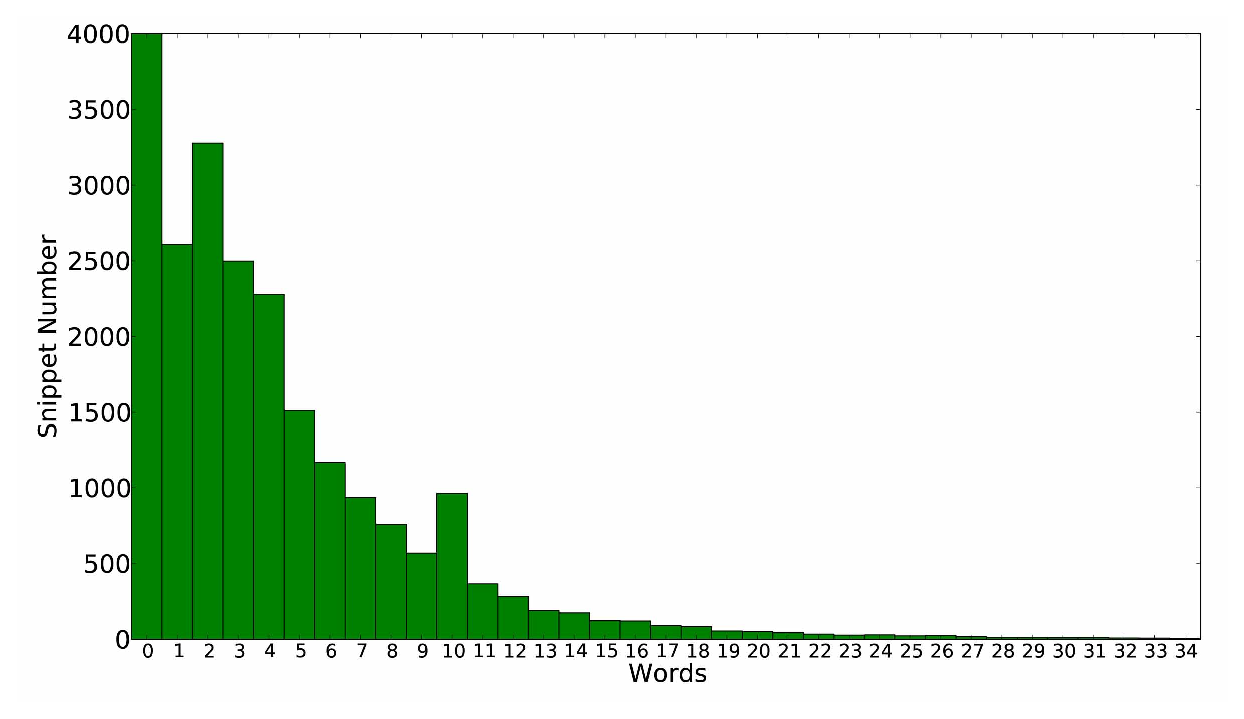
\includegraphics[height=1.3in,width=3.5in]{description.eps}
  \caption{提交到gist@GitHub和code@CSDN的代码片段描述长度}\label{snippet_description}
\end{figure}

\subsection{代码片段标签预测}
在实验中我们只使用Java语言的代码片段。我们的代码片段都是从code@CSDN中爬取的。我们随机选择了1515个Java代码片段然后对它们进行了手动本体术语标注。其中,有1345个代码片段用来训练分类模型然后剩余的170个用来测试该模型。在一系列参数的搜索后,在式(3)和式(4)中的参数$\alpha$,$\beta_d$和$\beta_c$被设置为2.2、0.5和0.5。

精确率和召回率是最常见的评估一个文本分类的标准。在代码注释这个环境下,精确率是指正确的注释个数除以总的搜索到的注释个数,召回率是指正确的注释个数除以总的正确的注释个数。精确率和召回率的公式为:

\begin{equation}\label{equ_precision}
    Precision=\frac{\sum_{i=1}^{N}{\frac{TP_i}{TP_i+FP_i}}}{N}
\end{equation}

\begin{equation}\label{equ_precision}
    Recall=\frac{\sum_{i=1}^{N}{\frac{TP_i}{TP_i+FN_i}}}{N}
\end{equation}

其中,N是指所有的测试代码片段数量。 $TP_i$是指True Positives,  $FP_i$是指False Positives, $FN_i$是指False Negatives。

结果如表~\ref{table_evaluation}所示。该表中D代表描述,P代表引用包,C代表源代码。

\begin{table}
  \centering
  \caption{使用不同的特征选择算法来对编程本体标注代码片段的评估结果}
  \begin{tabular}{c|c|c|c|c|c|c}
    \hline
  \multirow{2}{*}{Inputs} & \multicolumn{2}{c|}{MI}  &\multicolumn{2}{|c|}{IG}   &\multicolumn{2}{|c}{WFO}      \\
    \cline{2-7}
    &                 RC & PR        & RC & PR        & RC & PR            \\
    \hline
    D       & 88.43 & 84.13 & 86.76 & 80.23 & 86.76 & 80.52 \\
    D+P     & 89.31 & 84.33 & 87.94 & 80.62 & 87.90 & 80.92 \\
    D+C     & 91.07 & 85.15 & 88.23 & 79.12 & 88.23 & 80.01 \\
    P+C     & 58.72 & 47.89 & 64.70 & 54.35 & 64.70 & 54.07 \\
    D+P+C   & 91.37 & 84.56 & 88.23 & 79.12 & 88.23 & 79.96 \\
    \hline

    \hline
  \multirow{2}{*}{Inputs} & \multicolumn{2}{c|}{TFIDF}  &\multicolumn{2}{|c|}{WLLR}   &\multicolumn{2}{|c}{CHI}      \\
    \cline{2-7}
    &                 RC & PR        & RC & PR        & RC & PR            \\
    \hline
    D       & 72.64 & 72.50 & 86.07 & 83.94 & 47.94 & 45.52 \\
   D+P     & 72.05 & 71.91 & 87.25 & 85.11 & 48.52 & 45.52 \\
    D+C     & 62.05 & 62.35 & 87.84 & 84.92 & 46.17 & 43.29 \\
    P+C     & 43.53 & 44.11 & 61.17 & 50.52 & 35.58 & 31.51 \\
    D+P+C   & 62.05 & 62.35 & 88.43 & 85.50 & 46.17 & 43.37 \\
    \hline
  \end{tabular}
   \label{table_evaluation}
\end{table}

\end{CJK*}
\end{document}
